\documentclass[border=6pt]{standalone}
\usepackage{fontspec,unicode-math}
\setmainfont{Noto Serif}
\setmathfont{STIXTwoMath-Regular.otf}
\usepackage{tikz}
\usetikzlibrary{arrows.meta,calc,patterns,decorations.markings,decorations.pathmorphing,decorations.pathreplacing}
\tikzset{lev/.style={line width=1.2pt,line cap=butt},
 fine/.style={line width=.54pt},light/.style={line width=.37pt},
 curve/.style={line width=1.2pt,line cap=round,line join=round},
 ax/.style={line width=.62pt,-{Latex[length=2.1mm,width=1.15mm]}},
 ray/.style={line width=.58pt,-{Latex[length=1.85mm,width=.95mm]},shorten >=1.4pt,shorten <=1.4pt},
 dim/.style={line width=.52pt,{Latex[length=1.6mm,width=.85mm]}-{Latex[length=1.6mm,width=.85mm]}},
 flow/.style={line width=.60pt,postaction={decorate},decoration={markings,mark=at position .62 with {\arrow{Latex[length=1.8mm,width=.95mm]}}}},
 lab/.style={font=\fontsize{12}{14.4}\selectfont,inner sep=1.6pt},
 small/.style={font=\fontsize{10.5}{12.5}\selectfont,inner sep=1.3pt},
 tinylabel/.style={font=\fontsize{9.2}{11}\selectfont,inner sep=1.0pt},
 panel/.style={font=\fontsize{12}{14.4}\selectfont\itshape,inner sep=1.5pt}}
\pagestyle{empty}
\begin{document}
% CP15: author portrait sheet has less stretched vertical unit;
% x and y are independently scaled, while nodes retain legible font size.
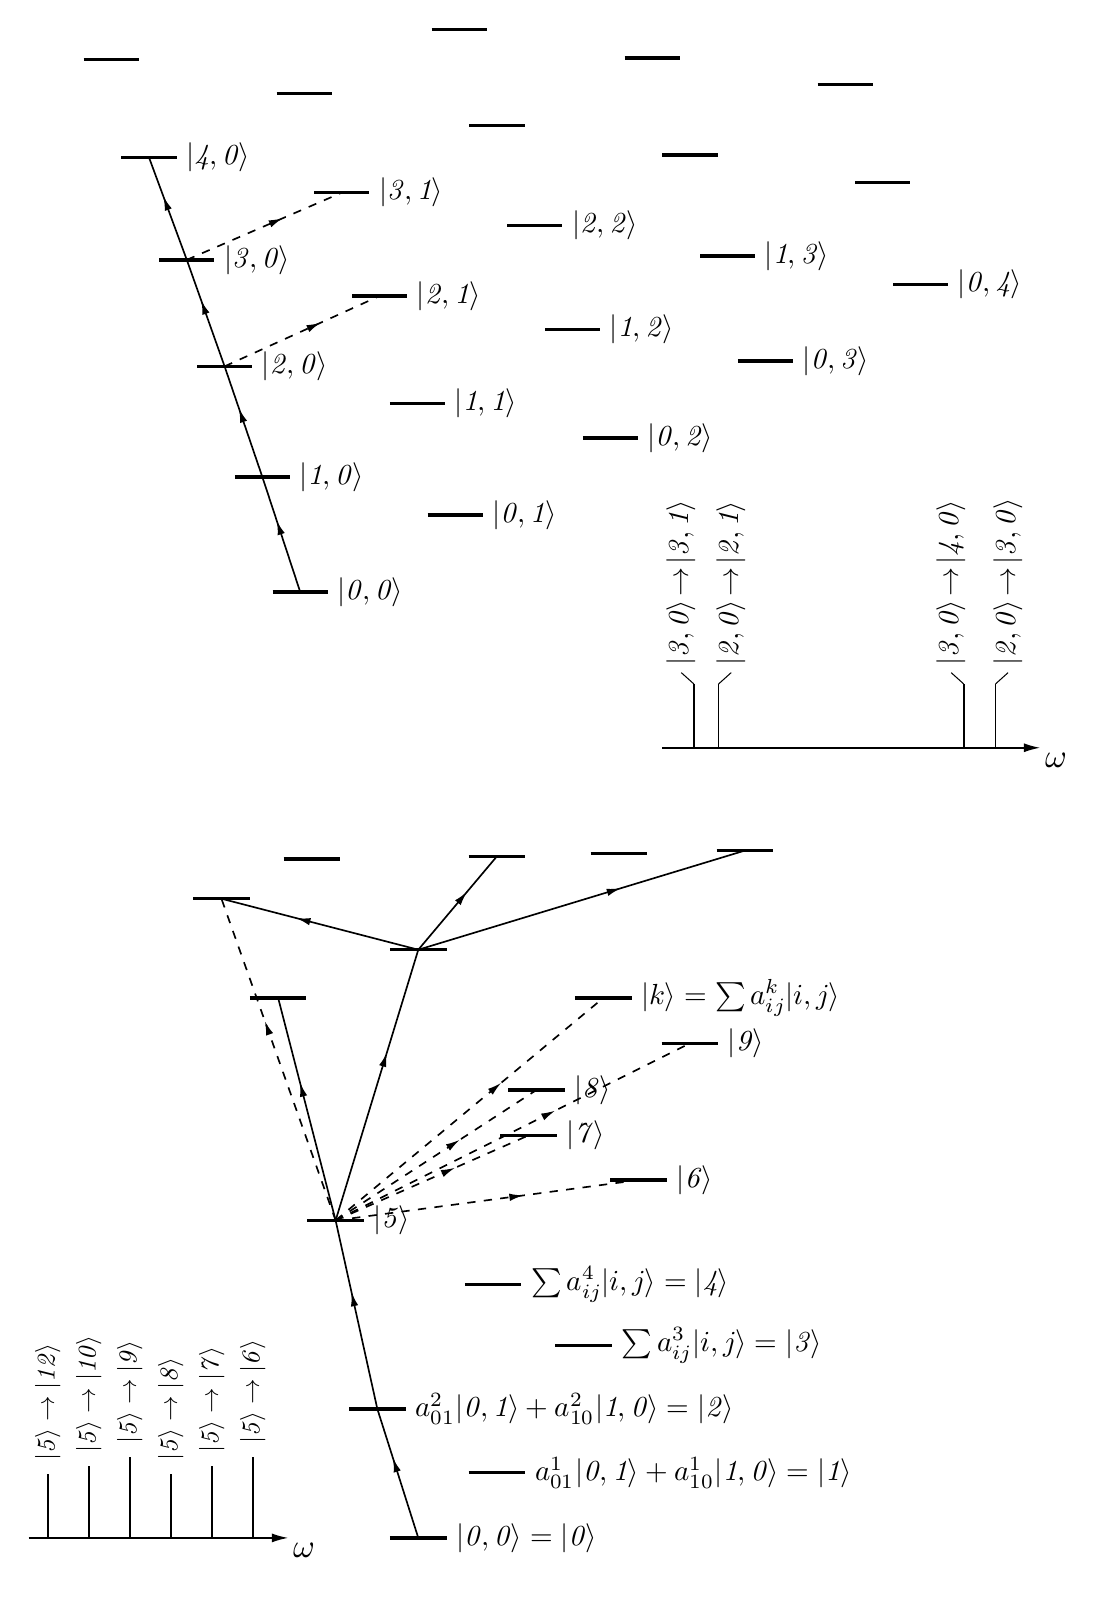
\begin{tikzpicture}[x=1cm,y=.90cm,line join=round]
\coordinate (a00) at (3.50000,14.15000);
\draw[lev] (3.15000,14.15000)--(3.85000,14.15000);
\node[small,anchor=west] at (3.92000,14.15000) {$|\mathit{0,0}\rangle$};
\coordinate (a10) at (3.02000,15.77000);
\draw[lev] (2.67000,15.77000)--(3.37000,15.77000);
\node[small,anchor=west] at (3.44000,15.77000) {$|\mathit{1,0}\rangle$};
\coordinate (a01) at (5.47000,15.23540);
\draw[lev] (5.12000,15.23540)--(5.82000,15.23540);
\node[small,anchor=west] at (5.89000,15.23540) {$|\mathit{0,1}\rangle$};
\coordinate (a20) at (2.54000,17.33168);
\draw[lev] (2.19000,17.33168)--(2.89000,17.33168);
\node[small,anchor=west] at (2.96000,17.33168) {$|\mathit{2,0}\rangle$};
\coordinate (a11) at (4.99000,16.81004);
\draw[lev] (4.64000,16.81004)--(5.34000,16.81004);
\node[small,anchor=west] at (5.41000,16.81004) {$|\mathit{1,1}\rangle$};
\coordinate (a02) at (7.44000,16.32080);
\draw[lev] (7.09000,16.32080)--(7.79000,16.32080);
\node[small,anchor=west] at (7.86000,16.32080) {$|\mathit{0,2}\rangle$};
\coordinate (a30) at (2.06000,18.83504);
\draw[lev] (1.71000,18.83504)--(2.41000,18.83504);
\node[small,anchor=west] at (2.48000,18.83504) {$|\mathit{3,0}\rangle$};
\coordinate (a21) at (4.51000,18.32636);
\draw[lev] (4.16000,18.32636)--(4.86000,18.32636);
\node[small,anchor=west] at (4.93000,18.32636) {$|\mathit{2,1}\rangle$};
\coordinate (a12) at (6.96000,17.85008);
\draw[lev] (6.61000,17.85008)--(7.31000,17.85008);
\node[small,anchor=west] at (7.38000,17.85008) {$|\mathit{1,2}\rangle$};
\coordinate (a03) at (9.41000,17.40620);
\draw[lev] (9.06000,17.40620)--(9.76000,17.40620);
\node[small,anchor=west] at (9.83000,17.40620) {$|\mathit{0,3}\rangle$};
\coordinate (a40) at (1.58000,20.28008);
\draw[lev] (1.23000,20.28008)--(1.93000,20.28008);
\node[small,anchor=west] at (2.00000,20.28008) {$|\mathit{4,0}\rangle$};
\coordinate (a31) at (4.03000,19.78436);
\draw[lev] (3.68000,19.78436)--(4.38000,19.78436);
\node[small,anchor=west] at (4.45000,19.78436) {$|\mathit{3,1}\rangle$};
\coordinate (a22) at (6.48000,19.32104);
\draw[lev] (6.13000,19.32104)--(6.83000,19.32104);
\node[small,anchor=west] at (6.90000,19.32104) {$|\mathit{2,2}\rangle$};
\coordinate (a13) at (8.93000,18.89012);
\draw[lev] (8.58000,18.89012)--(9.28000,18.89012);
\node[small,anchor=west] at (9.35000,18.89012) {$|\mathit{1,3}\rangle$};
\coordinate (a04) at (11.38000,18.49160);
\draw[lev] (11.03000,18.49160)--(11.73000,18.49160);
\node[small,anchor=west] at (11.80000,18.49160) {$|\mathit{0,4}\rangle$};
\coordinate (a50) at (1.10000,21.66680);
\draw[lev] (0.75000,21.66680)--(1.45000,21.66680);
\coordinate (a41) at (3.55000,21.18404);
\draw[lev] (3.20000,21.18404)--(3.90000,21.18404);
\coordinate (a32) at (6.00000,20.73368);
\draw[lev] (5.65000,20.73368)--(6.35000,20.73368);
\coordinate (a23) at (8.45000,20.31572);
\draw[lev] (8.10000,20.31572)--(8.80000,20.31572);
\coordinate (a14) at (10.90000,19.93016);
\draw[lev] (10.55000,19.93016)--(11.25000,19.93016);
\coordinate (a42) at (5.52000,22.08800);
\draw[lev] (5.17000,22.08800)--(5.87000,22.08800);
\coordinate (a33) at (7.97000,21.68300);
\draw[lev] (7.62000,21.68300)--(8.32000,21.68300);
\coordinate (a24) at (10.42000,21.31040);
\draw[lev] (10.07000,21.31040)--(10.77000,21.31040);
\draw[flow] (a00)--(a10);
\draw[flow] (a10)--(a20);
\draw[flow] (a20)--(a30);
\draw[flow] (a30)--(a40);
\draw[flow,dashed] (a20)--(a21);
\draw[flow,dashed] (a30)--(a31);
\draw[ax] (8.10000,11.95000)--(12.90000,11.95000);
\node[lab,anchor=north west] at (12.90000,11.95000) {$\omega$};
\draw[fine] (8.50000,11.95000)--(8.50000,12.85000);
\draw[light] (8.50000,12.85000)--(8.34000,13.01000);
\node[small,anchor=west,rotate=90] at (8.34000,13.05000) {$|\mathit{3,0}\rangle\!\to\!|\mathit{3,1}\rangle$};
\draw[fine] (8.81360,11.95000)--(8.81360,12.85000);
\draw[light] (8.81360,12.85000)--(8.97360,13.01000);
\node[small,anchor=west,rotate=90] at (8.97360,13.05000) {$|\mathit{2,0}\rangle\!\to\!|\mathit{2,1}\rangle$};
\draw[fine] (11.92720,11.95000)--(11.92720,12.85000);
\draw[light] (11.92720,12.85000)--(11.76720,13.01000);
\node[small,anchor=west,rotate=90] at (11.76720,13.05000) {$|\mathit{3,0}\rangle\!\to\!|\mathit{4,0}\rangle$};
\draw[fine] (12.33040,11.95000)--(12.33040,12.85000);
\draw[light] (12.33040,12.85000)--(12.49040,13.01000);
\node[small,anchor=west,rotate=90] at (12.49040,13.05000) {$|\mathit{2,0}\rangle\!\to\!|\mathit{3,0}\rangle$};
\node[panel] at (6.50000,11.10000) {а};
\coordinate (b0) at (5.00000,0.80000);
\draw[lev] (4.64000,0.80000)--(5.36000,0.80000);
\node[small,anchor=west] at (5.43000,0.80000) {$|\mathit{0,0}\rangle=|\mathit0\rangle$};
\coordinate (b1) at (6.00000,1.72000);
\draw[lev] (5.64000,1.72000)--(6.36000,1.72000);
\node[small,anchor=west] at (6.43000,1.72000) {$a^1_{01}|\mathit{0,1}\rangle+a^1_{10}|\mathit{1,0}\rangle=|\mathit1\rangle$};
\coordinate (b2) at (4.48000,2.62000);
\draw[lev] (4.12000,2.62000)--(4.84000,2.62000);
\node[small,anchor=west] at (4.91000,2.62000) {$a^2_{01}|\mathit{0,1}\rangle+a^2_{10}|\mathit{1,0}\rangle=|\mathit2\rangle$};
\coordinate (b3) at (7.10000,3.52000);
\draw[lev] (6.74000,3.52000)--(7.46000,3.52000);
\node[small,anchor=west] at (7.53000,3.52000) {$\sum a^3_{ij}|i,j\rangle=|\mathit3\rangle$};
\coordinate (b4) at (5.95000,4.38000);
\draw[lev] (5.59000,4.38000)--(6.31000,4.38000);
\node[small,anchor=west] at (6.38000,4.38000) {$\sum a^4_{ij}|i,j\rangle=|\mathit4\rangle$};
\coordinate (b5) at (3.95000,5.28000);
\draw[lev] (3.59000,5.28000)--(4.31000,5.28000);
\node[small,anchor=west] at (4.38000,5.28000) {$|\mathit5\rangle$};
\coordinate (b6) at (7.80000,5.85000);
\draw[lev] (7.44000,5.85000)--(8.16000,5.85000);
\node[small,anchor=west] at (8.23000,5.85000) {$|\mathit6\rangle$};
\coordinate (b7) at (6.40000,6.48000);
\draw[lev] (6.04000,6.48000)--(6.76000,6.48000);
\node[small,anchor=west] at (6.83000,6.48000) {$|\mathit7\rangle$};
\coordinate (b8) at (6.50000,7.12000);
\draw[lev] (6.14000,7.12000)--(6.86000,7.12000);
\node[small,anchor=west] at (6.93000,7.12000) {$|\mathit8\rangle$};
\coordinate (b9) at (8.45000,7.78000);
\draw[lev] (8.09000,7.78000)--(8.81000,7.78000);
\node[small,anchor=west] at (8.88000,7.78000) {$|\mathit9\rangle$};
\coordinate (b10) at (7.35000,8.42000);
\draw[lev] (6.99000,8.42000)--(7.71000,8.42000);
\node[small,anchor=west] at (7.78000,8.42000) {$|k\rangle=\sum a^k_{ij}|i,j\rangle$};
\coordinate (b11) at (3.22000,8.42000);
\draw[lev] (2.86000,8.42000)--(3.58000,8.42000);
\coordinate (b12) at (5.00000,9.10000);
\draw[lev] (4.64000,9.10000)--(5.36000,9.10000);
\coordinate (b13) at (2.50000,9.82000);
\draw[lev] (2.14000,9.82000)--(2.86000,9.82000);
\coordinate (b14) at (3.65000,10.38000);
\draw[lev] (3.29000,10.38000)--(4.01000,10.38000);
\coordinate (b15) at (6.00000,10.42000);
\draw[lev] (5.64000,10.42000)--(6.36000,10.42000);
\coordinate (b16) at (7.55000,10.46000);
\draw[lev] (7.19000,10.46000)--(7.91000,10.46000);
\coordinate (b17) at (9.15000,10.50000);
\draw[lev] (8.79000,10.50000)--(9.51000,10.50000);
\draw[flow] (b0)--(b2);
\draw[flow] (b2)--(b5);
\draw[flow] (b5)--(b11);
\draw[flow] (b5)--(b12);
\draw[flow] (b12)--(b13);
\draw[flow] (b12)--(b15);
\draw[flow] (b12)--(b17);
\draw[flow,dashed] (b5)--(b6);
\draw[flow,dashed] (b5)--(b7);
\draw[flow,dashed] (b5)--(b8);
\draw[flow,dashed] (b5)--(b9);
\draw[flow,dashed] (b5)--(b10);
\draw[flow,dashed] (b5)--(b13);
\draw[ax] (0.05000,0.80000)--(3.35000,0.80000);
\node[lab,anchor=north west] at (3.35000,0.80000) {$\omega$};
\draw[fine] (0.30000,0.80000)--(0.30000,1.70000);
\node[tinylabel,anchor=west,rotate=90] at (0.30000,1.84000) {$|\mathit5\rangle\to|\mathit{12}\rangle$};
\draw[fine] (0.82000,0.80000)--(0.82000,1.82000);
\node[tinylabel,anchor=west,rotate=90] at (0.82000,1.96000) {$|\mathit5\rangle\to|\mathit{10}\rangle$};
\draw[fine] (1.34000,0.80000)--(1.34000,1.94000);
\node[tinylabel,anchor=west,rotate=90] at (1.34000,2.08000) {$|\mathit5\rangle\to|\mathit{9}\rangle$};
\draw[fine] (1.86000,0.80000)--(1.86000,1.70000);
\node[tinylabel,anchor=west,rotate=90] at (1.86000,1.84000) {$|\mathit5\rangle\to|\mathit{8}\rangle$};
\draw[fine] (2.38000,0.80000)--(2.38000,1.82000);
\node[tinylabel,anchor=west,rotate=90] at (2.38000,1.96000) {$|\mathit5\rangle\to|\mathit{7}\rangle$};
\draw[fine] (2.90000,0.80000)--(2.90000,1.94000);
\node[tinylabel,anchor=west,rotate=90] at (2.90000,2.08000) {$|\mathit5\rangle\to|\mathit{6}\rangle$};
\node[panel] at (6.50000,0.12000) {б};
\end{tikzpicture}
\end{document}
